% !TeX root = ../thesis.tex
%
\setcounter{chapter}{4}
\chapter{Fostering Computational Thinking Skills through Gameplay}\label{chap:tapasplay}

\cleanchapterquote{You'll never see a video game being advertised as being easy. Children who do not like school will tell you it’s not because it’s too hard. It's because it's boring.}{Seymour Papert}{The Children's Machine, 1993}

The previous chapter focused on using a \ac{TUI} to foster \ac{CT} skills in a specific application domain, namely \ac{IL} environments, where learning is mostly self-directed and takes place as people go about their daily activities, driven by their preferences and intentions. This chapter deals with exploiting a \ac{TUI} to support the development of \ac{CT} skills in \ac{IL} domains in combination with gameplay activities.

\section{Introduction}
\deleted[comment={MP5, D34}]{As discussed in the first chapter, being able to understand and trust algorithmic solutions, and to participate in the design and development of such solutions can bring several benefits in everyday life, making everyone able to succeed in today's complex and technological society~\cite{Bundy:2007}.}

\deleted{These skills are not confined to the programming realm though, as they enable people to acquire a new way of thinking and looking at the world, not just related to developing software, fostering the so-called \ac{CT} skills, i.e.\ abilities like problem-solving, abstraction, and pattern recognition to name but a few. They allow breaking problems down into small chunks and abstract unnecessary details and enabling them to be expressed on a computer to ease the process of finding their solutions~\cite{Vee:2013wc}.}

\deleted{\ac{CT} is a recent notion, which was introduced by Seymour Papert in~\cite{Papert:1980uh}, before Jeannette Wing discussed it widely for the first time in her seminal work~\cite{Wing:2006iz}. Since then, many scholars have tried to define it and find a solid way to assess the set of skills that make it up. According to Wing and other research scholars, is mostly about problem-solving, while abstraction and algorithmic thinking are regarded in~\cite{Wing:2010} as highly relevant thought processes.}

\deleted{Therefore, \ac{CT} skills should become an important piece of end-users' background, like reading, writing and calculating. In line with this consideration, several initiatives all over the world are aimed at ensuring that students develop \ac{CT} skills at the K-12 level~\cite{Lee:2014er,Yadav:2014,Voogt:2015}.}

\deleted{Since \ac{CT} skills are usually recognized as typical of programmers and software designers, most of the approaches to teaching such skills involve \ac{VPL} (e.g.,~\cite{Resnick:2009bd}) or game design activities (e.g.,~\cite{Repenning:2000}) aimed at teaching the concepts underlying imperative programming (such as symbolic representation, conditionals, loops, operators, etc.). }

\deleted{However, as stated by Wing, \ac{CT} goes beyond programming, since it fosters the creation of a new mindset oriented towards problem-solving, thanks to the ability to think at different levels of abstraction and at decomposing problems into sub-problems. In other words, \ac{CT} should focus on ``conceptualizing'' rather than ``programming''~\cite{Wing:2006iz}.}

\deleted{By looking at new and engaging ways of promoting \ac{CT} skills to new audiences, one might turn to the constructivist theories of Jean Piaget~\cite{Piaget:1969vq}: he suggested that exploiting human's innate dexterity for objects manipulation in the physical world and its afforded social interactions could be an effective way of supporting experiential learning of abstract concepts, such as the ones underpinning \ac{CT}. This concept sits at the core of \acp{TUI}, a digital interaction paradigm aiming at providing users with an easy to use interface, often used to support the interaction of young children with technology in the classroom. Such paradigm might be able to foster \ac{CT} skills by supporting users with a concrete representation of the concepts it involves and provide a tool supporting its collaborative learning~\cite{McNerney:2004jc,Horn:2009be}.}

\deleted[comment={D1, D34, D35}]{To recap, from this context discerns the main Research Question addressed by this thesis: \textit{``Can the collaborative and cognitive naturalness of physical objects manipulation at the basis of \acp{TUI} aid the understanding of core algorithmic principles and thus improve \ac{CT} skills?''}.}

\replaced{As briefly mentioned in the first chapter, e}{E}nhancing support for cultivating users' \ac{CT} skills --- and more generally their usual learning experiences --- can be optimal when tools and activities are able to keep them in the so-called ``Flow state'': according to Csikszentmihalyi's theory~\cite{nakamura2014concept}, it refers to a state of intense concentration, sustained interest, and enjoyment of the challenge of an activity, when skill level and challenge level of a task are at their highest, allowing users to learn at intense focus. It is hard to obtain such balance, since too much challenge causes anxiety, whereas too little challenge leads to boredom; one of the most common and explored ways of keeping learners in such state is through gameplay, that is by providing them with an engaging challenge and real-time feedback in response to their choices.

Coupling such activities able to keep learners in the Flow state with physical interaction might enhance even further learning of \ac{CT} skills by leveraging on a sustained engagement level, afforded social interactions, and a concrete representation of the abstract concepts underpinning it.

The Research Question derived from this context and addressed by this chapter is then: \textit{``Can physical objects manipulation provide a playful and engaging way of learning \ac{CT} skills through gameplay?''}.

The hypothesis is that through the design of an appropriate gameplay involving \acp{TUI} and an engaging medium like \ac{VR}, a high efficacy in supporting \ac{CT} skills can be achieved. Furthermore, using a digital shared surface with tangibles might foster collaborative learning\added[comment={D36}]{~\cite{Subramanian:2007kx}} and physical interaction to further improve \ac{CT} skills.

The hypothesis was tested by involving 18 UK secondary school Key Stage 4 (15 years old) female students in collaborative gaming sessions with a prototype of a game called TAPASPlay. The young girls had no previous programming experience and only a small group had some previous experience programming with Scratch.

\deleted[comment={D37}]{Focusing on young girls allowed to test the level of engagament the platform could provide; it is well known that gender imbalance affects the tech industry and the gaming world specifically~\cite{tzafilkou2017gender,beckwith2006gender,Huff:2002:GSD:543812.543842,Cassell:1998:BMK:295056}, indeed the majority of game players are males. Demonstrating that the platform provides a collaborative, playful and engaging experience teaching \ac{CT} skills to young girls can contribute to widening end-users' participation in system design and development both in terms of involvement and gender balance.}

The chapter concludes with a set of observations and recommendations for designing payful and engaging systems to teach \ac{CT} skills to a wide audience.

\section{Related Works}
Digital games proved attractive and engaging for all groups of people and therefore, \ac{GBL} has been proposed as one pedagogical framework for developing \ac{CT} skills~\cite{Weintrop:2016vc}. In order to help to acquire \ac{CT} skills two main approaches have been introduced in \ac{GBL}: learning through designing games and learning through gameplay.

\subsection{Learning through Design}
Learning through designing games has been studied for many years. In 1996 AgentSheets, designed by Alexander Repenning, was released, even though the first prototype dates back to 1989~\cite{Repenning:2000}. AgentSheets is still used in multiple contexts, from middle to high schools to academic environments, for various purposes such as introducing to programming, supporting storytelling and prototyping simple games. The tool takes its name from the fact that the user develops the program on a grid resembling a spreadsheet, whose cells contain agents. These entities, visualized as pictures, can perform multiple actions like reading Web pages or playing sounds and animations. A graphical interface allows creating ``if-then'' rules that represent agents' behaviour. Drag-and-drop interaction is supported, which revealed to be an interaction style suitable to people without any programming background. It has been demonstrated that AgentSheets favours \ac{CT} skills like problem-solving, abstraction, and pattern recognition~\cite{Koh:2010}. Monteiro et al.~\cite{Monteiro:2017} have recently studied how AgentSheets may improve algorithm design skills, thanks to the logic underlying the creation of rules, as well as teach the automation concept. 

Alice is another \ac{VPE}, developed at the Carnegie Mellon University starting from 1997~\cite{Herbert:2012}. It focuses on creating 3D programming projects and is actually an object-based programming language that allows creating animations and interactive games by defining object behaviour through a drag-and-drop interaction of specific blocks. Alice is a valid tool for supporting storytelling while being exposed to basic programming concepts, both of imperative and object-oriented programming paradigms, without the burden of remembering syntactic constructs. 
Alice has been successfully employed to assess \ac{CT} skills in primary and middle school~\cite{Wang:2014jy,Werner:2012}.

Similarly, Kodu is an integrated \ac{VPE} which allows creating games structured as 3D worlds comprising different types of objects able to react to some events~\cite{Fowler:2012}. Kodu is aimed at fostering familiarity with basic programming notions, in an intuitive and playful way. It thus supports notions of the imperative programming paradigms, such as sequentiality, conditional instructions, variables and assignments; it also encompasses some concepts of object-oriented programming, such as that of classes and objects, and information hiding. Different studies have been performed to demonstrate the capability of Kodu to improve \ac{CT} skills such as problem-solving, abstraction, problem decomposition and pattern recognition~\cite{Fowler:2011,Touretzky:2013}.

Perhaps the most influential and versatile tool for learning how to program by designing games is Scratch~\cite{Resnick:2009bd}, developed at the MIT and publicly released for the first time in 2005. It is a \ac{VPL} whose interaction is made simple thanks to draggable instructions represented by blocks, fitting one another like puzzle pieces. The process of assembling instructions is guided by the different shapes and colours of blocks, suggesting which constraints must be satisfied. One of its biggest strengths is the large and heterogeneous community of users that, combined with the possibility of reusing and remixing other users' code, permits to cooperate, share knowledge and realize complex projects more easily. Scratch is widely considered a successful tool to teach programming to K-12 students and foster \ac{CT} skills~\cite{Brennan:2012,Cetin:2016,Grover:2015}.

Robot programming has regarded itself as game-design learning; for instance, in~\cite{Atmatzidou:2016} Lego Mindstorms~\cite{MINDSTORMS} is used to improve \ac{CT} skills of high school students. In this approach, the learner first identifies the goal for the robot and then defines an algorithm, that is, a set of steps to carry out, to accomplish the goal; then the robot can follow the instructions and act accordingly; the learner may debug the program by observing and tuning robot's behaviour.

Tangible Programming is yet another way to create interactive games by mixing physical objects with a more traditional instruction-based approach. For example, in Tern~\cite{Horn:2007} the goal of introducing children to computer programming is pursued by using small wooden cubes with instructions on their faces. The sequence of instructions results in a series of movements performed by a small robot. In T-Maze~\cite{Wang:2011} the programming phase is conducted in a very similar fashion, with a camera dedicated to reading the programming sequence in real-time. Children from 5 to 9 can create their own maze maps and complete escaping tasks, thus \replaced[comment={D39}]{solving}{accomplishing} simple programming tasks\deleted{ in a positive way}.

\subsection{Learning through Gameplay}
Learning through gameplay is another approach to \ac{GBL} for improving \ac{CT} skills. It might represent a valid alternative to learning through design, since, as highlighted in~\cite{Lee:2014er}, building a game from scratch could be too challenging for novice programmers and thus frustrating for the majority of players.

Among them,~\cite{Kazimoglu:2012ft} proposes Program Your Robot, a game prototype developed to support children in practising the five skills that the authors identified as fundamental for \ac{CT}: problem-solving, algorithm design, debugging, simulation and socializing. It is a puzzle-solving game in which the player has to assist a simulated robot to reach a certain point on a grid. Players thus design a solution algorithm that the robot will follow, by using symbolic representations of ``action commands'' (to move the robot in an environment) and ``programming commands'' (basic constructs such as sequence, selection, iteration, and function). These commands are dragged from their toolbars to specific areas of the environment. Players need to move the robot, activate lights and collect items by proceeding towards different levels of the game. Rewards are obtained in the form of new collectible items, slots or enemies to avoid as the player advances through the game. Program Your Robot is conceived as a serious game and thus differs from the software applications for game design mentioned before, which can be deemed programming languages to all effects. Indeed, tools like AgentSheets or Scratch were designed in order to teach the basics of programming and to show how fun it can be. Instead, Kazimoglu et al.~\cite{Kazimoglu:2012ft} were moved by the goal of creating a game that could foster \ac{CT} skills.
However, also in Program Your Robot the player is exposed to basic programming constructs and thus the gameplay keeps on being strictly related to a programming activity. 

CTArcade~\cite{Lee:2014er} is another serious game where players have to design a set of rules that are executed by a character while playing Tic-Tac-Toe. Making these rules explicit is considered an important process, because people often apply them in a natural, perhaps unconscious way and normally there is neither the chance nor the reason to transform this knowledge into abstract instructions. Lee et al.~\cite{Lee:2014er} report a study, implementing a ``think aloud'' protocol, where 18 children have been observed playing on CTArcade and on paper; the study shows that children articulate more \ac{CT} skills (problem decomposition, pattern recognition, pattern generalization and algorithmic thinking) using CTArcade compared to playing on paper. However, the analysis was carried out on Tic-Tac-Toe only, a widely popular and common game; therefore, \ac{CT} was difficult to externalize and observe.

Liu et al.~\cite{Liu:2011} investigate the use of TrainB\&P to assist students in developing computational problem-solving abilities. With this simulation game, the students can construct a railway system and design the transportation behaviours of trains on a railway by using several building blocks such as straight, curved, and branch tracks. In particular, the system allows students to program the transportation behaviours and simulate them in a 3D environment. The results of the study, carried out with the participation of 117 students, demonstrate how the gameplay enhances students' motivation and brings them in a flow state during the learning experience. 

All the above systems use traditional interaction styles based on keyboard and mouse; on the contrary, even though TAPASPlay shares with them the objective of fostering \ac{CT} skills through gameplay, it leverages on an interaction style based on tangible objects and \ac{VR}. Tangible interaction and \ac{VR} have been chosen to \added[comment={D40}]{try and }increase the playfulness of the system and create an engaging and collaborative learning environment. Furthermore, as investigated in the previous chapter, physical object manipulation might help users deal with abstract concepts, as well as cultivate skills such as abstraction and problem decomposition~\cite{Wang:2014jy}. In line with~\cite{kafai:2016}, TAPASPlay also aims to foster collaborative learning, that is, it regards \ac{CT} as a creative and social practice\added[comment={D41}]{ (the ``Connecting'' Perspective defined in Brennan and Resnick's Framework~\cite{Brennan:2012})}. Lastly, TAPAS\-Play fits with\-in the realm of Con\-struc\-tion\-ist Vid\-e\-o Games~\cite{Weintrop:2016vc}, name\-ly com\-pu\-ta\-tion\-al en\-vi\-ron\-ments in which play\-ers cre\-ate per\-son\-al\-ly mean\-ing\-ful ar\-te\-facts to o\-ver\-come ar\-ti\-fi\-cial con\-flicts or ob\-sta\-cles re\-sult\-ing in quan\-ti\-fi\-a\-ble out\-comes. In the fol\-low\-ing, the de\-sign and im\-ple\-men\-ta\-tion of TAPAS\-Play is de\-scribed in de\-tail. 

\section{TAPASPlay}\label{sec:tapasplay}
TAPASPlay is a turn-taking game intended for end-users with little or no experience in programming, designed to foster their \ac{CT} abilities by leveraging on physical interaction and keeping them engaged in a Flow state.

\subsection{Design}
TAPASPlay has been developed on top of the \acr{TAPAS} system discussed in the previous chapter; it is a block-based programming environment that allows end-users to build simple workflows by assembling different services with the aim of fostering \ac{CT} skills in \ac{IL} scenarios. The interaction with \ac{TAPAS} is carried out using smartphones as tangible objects and digital blocks projected over a tabletop surface.

As in \ac{TAPAS}, interacting with TAPASPlay requires a tabletop surface, an RGB camera and a smartphone. Smartphone movements on the display or surface are tracked by the RGB camera, which locates the position of a fiducial marker shown on the phone screen and uses it as reference point. TAPASPlay has been implemented as a Web application that is projected on the tabletop surface and is able to interact with players' smartphones. A smartphone application provides players with additional feedback and tools for completing the game. Finally, \ac{VR} technology is used to visualize the outcome of the game.

As mentioned earlier, TAPASPlay can be regarded as a constructionist video game aimed at providing users with an educational and entertaining experience. \replaced[comment={D42}]{It aims at}{The former has the goal of} teaching \ac{CT} skills through gameplay\replaced{ while}{, the latter has the goal of} fostering socialization and thus collaborative learning.

To accomplish these goals, the game has been designed on the basis of the following requirements:
\begin{enumerate}
\item The interaction with the game should be based on a puzzle metaphor that proved to be an intuitive approach to find a solution to a given problem (algorithmic thinking)~\cite{turchi2017tapas}. This means that TAPASPlay has to communicate the existence of constraints and to support the gameplay through puzzle pieces and their shapes, aiding users whilst giving constraints in their selection process.
\item Puzzle pieces should be physically manipulated, in order to favor the appropriation of abstract concepts through tangible interaction~\cite{Wang:2014jy}.
\item The game must be played in player versus player modality, since competition is one of the most important elements of serious games to increase motivation and learning~\cite{Cagiltay:2015}. Moreover, each character might be programmed by a group of players, thus favoring socialization and collaboration within the group. 
\item The game must feature a storytelling suitable to a \ac{VR} representation, which can be visualized by wearing affordable goggles (e.g., Google Cardboard~\cite{CARDBOARD}).
\end{enumerate}

These requirements led to conceive gameplay around alchemy, that is the (fictitious) process of transmuting metals: players compete to be the best alchemist by forging three swords and three shields, made of three different metals. In order to build each sword, players have a limited amount of energy points they can spend on transmutations, which in turn make a sword earn force points. Transmutations (also called transformations in the following) can be combined together in different ways, allowing users to experiment and practice problem abstraction and decomposition by following the puzzle constraints. The objective is to maximise force points while carefully managing energy points on each sword. Trying to earn force points while finding a tradeoff with energy points is an {\rmfamily NP}-hard problem that can be solved with different strategies (e.g., greedy algorithm, backtracking), requiring algorithmic thinking in finding even a sub-optimal solution.

In particular, the game is structured in three phases:
\begin{enumerate}
\item defining the offensive strategies, by means of forging swords;
\item defining the defensive strategies, by means of forging shields;
\item visualizing the representation of a battle in a \ac{VR} headset.
\end{enumerate}

\subsection{Forging Swords}\label{sec:swords}
The first phase is aimed at fostering different \ac{CT} skills, such as problem decomposition, algorithmic thinking, abstraction, and iteration. During the first phase, each player creates three offensive strategies by composing three different swords. In order to accomplish that, players have to attach transformations, represented as pieces of a puzzle, to a halo surrounding the user's smartphone on the main display. Each strategy is a sequence of transformations taken from a randomly generated set shown at the beginning of the game on the main display (figure~\ref{fig:1}).

\begin{figure}[ht!]
  \centering
  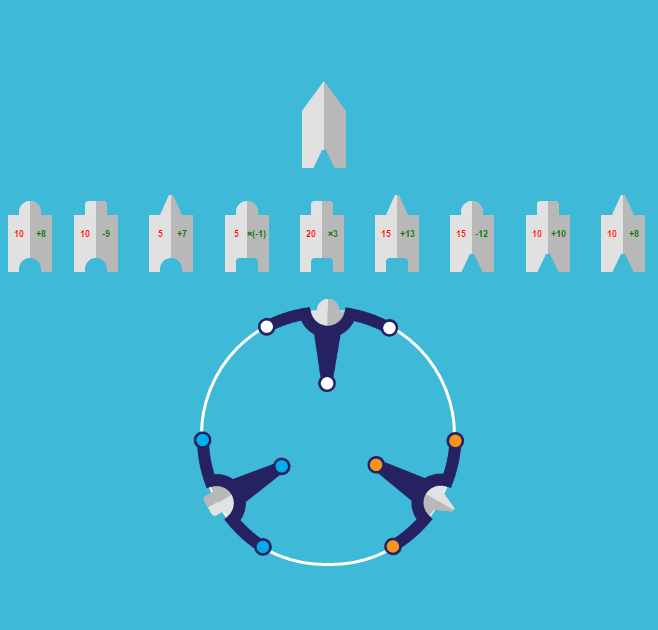
\includegraphics[width=.7\textwidth]{images/c5/starting-state.png}
  \caption{Initial state of the game: the set of transformations is displayed, as well as the main halo with three hilts and the final piece.}\label{fig:1}
\end{figure}

Each half of the tabletop screen is available for a player to forge the swords. The halo, with its three hilts, follows the movement of the dragged smartphone and, when a collision with a puzzle piece is detected, such \added[comment={D44}]{a }piece is attached to the vertically oriented hilt given that the move is allowed by the game rules. The three swords are defined one at a time, so that each can have a different set of puzzle pieces available for the players, avoiding repetitions and increasing in difficulty. For instance, in figure~\ref{fig:2}, players are creating their first swords.

\begin{figure}[ht!]
  \centering
  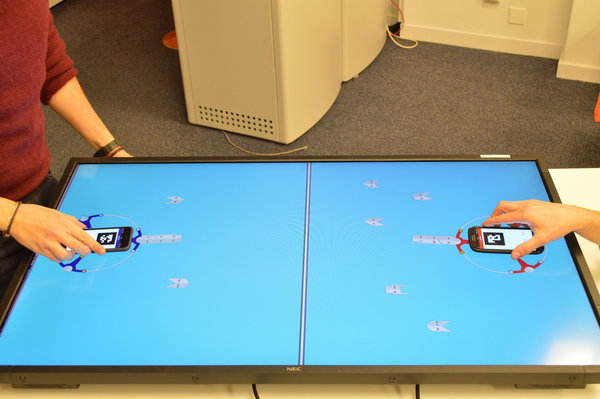
\includegraphics[width=.7\textwidth]{images/c5/tangible-interaction.png}
  \caption{Forging swords through tangible and puzzle-like interaction.}\label{fig:2}
\end{figure}

A hilt attached to the main halo surrounding the player’s smartphone represents the starting point of the sword (figure~\ref{fig:3a}), while the final piece has a shape that resembles the tip (figure~\ref{fig:3b}).

\begin{figure}[ht!] 
  \begin{subfigure}[t]{0.48\linewidth}
    \centering
    
\includegraphics[width=0.75\linewidth]{images/c5/hilt.png} 
    \caption{An example of initial state of the sword.}\label{fig:3a}
  \end{subfigure}\hfill
  \begin{subfigure}[t]{0.48\linewidth}
    \centering
    
\includegraphics[width=0.35\linewidth]{images/c5/final-piece.png} 
    \caption{An example of final piece.}\label{fig:3b}
  \end{subfigure}
  \caption{Examples of initial and final pieces of a sword.}
\end{figure}

Every puzzle piece has an input and an output shape. There are three shapes in total, round, square and triangular, which in turn correspond to three types of metal, namely bronze, iron, and steel. So, if a puzzle piece has a round input shape and a triangular output shape as in figure~\ref{fig:4a}, it is equivalent to a transformation that turns bronze into steel. Each sword is made of a different type of metal, determined by the shape of the final puzzle piece. For example, in figure~\ref{fig:4b} the shape of the final piece is triangular and thus a steel sword has been forged.

The aim of this first phase is to maximize the force points of each sword, which can be earned by attaching transformations to the sequence. However, every transformation consumes a number of energy points. More precisely, a transformation is a tuple of four values:
\begin{enumerate*}[label=(\arabic*)]
  \item an input shape,
  \item an output shape,
  \item a number of energy points, displayed on the transformation (left half in figure~\ref{fig:4a}), and
  \item the force points gained, displayed on the transformation as well (right half in figure~\ref{fig:4a}).
\end{enumerate*}

In order to apply a transformation, two conditions need to be fulfilled:
\begin{enumerate*}[label=(\arabic*)]
  \item the input shape of the transformation is the same as the output shape of the last transformation attached to the sword (or, if the transformation applied is the first one, the input shape has to be the same as the output shape of the initial state of the sword); and
  \item the alchemist must have a number of energy points greater or equal than the one shown on the transformation.
\end{enumerate*}

Once a transformation is applied (supported by a ``magnetic effect'' on the puzzle piece provided by the system), the energy points of the alchemist are decreased by the energy points of the transformation, while the force points of the strategy can be increased, decreased or multiplied, depending on the operation suggested by the transformation.

The initial state of each sword consists of an output shape attached to a hilt on the halo, a number of force points, and a number of energy points. The final state (figure~\ref{fig:4b}) is reached when the player is satisfied with its sequence of transformations and decides to --- and can --- attach the final piece to the sword. 

\begin{figure}[ht!] 
  \begin{subfigure}[t]{0.48\linewidth}
    \centering
    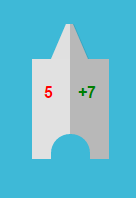
\includegraphics[width=0.35\linewidth]{images/c5/transformation.png} 
    \caption{An example transformation.}\label{fig:4a}
  \end{subfigure}\hfill
  \begin{subfigure}[t]{0.48\linewidth}
    \centering
    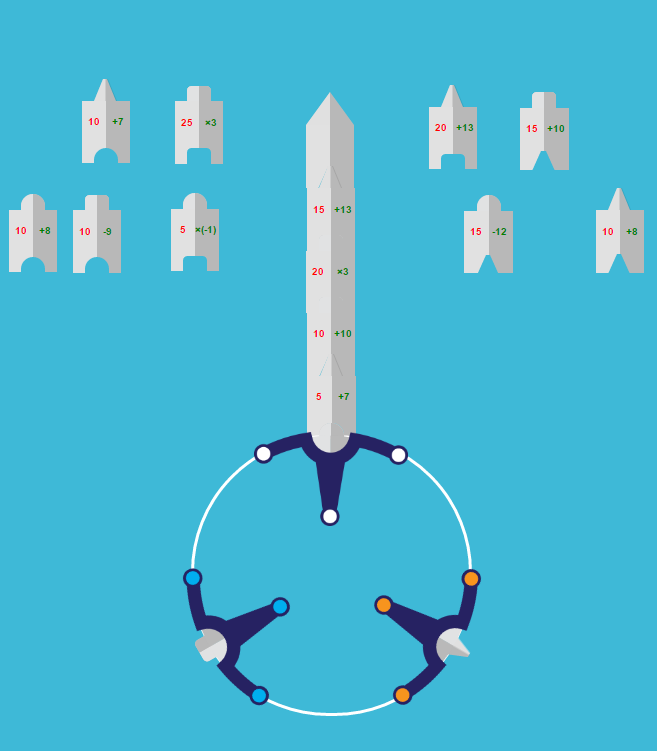
\includegraphics[width=0.60\linewidth]{images/c5/sword-example.png} 
    \caption{A sword example.}\label{fig:4b}
  \end{subfigure}
  \caption{Forging a sword by composing transformations.}
\end{figure}

Players can see a feedback of their operation on their smartphone since force and energy points presented on their screen are updated according to the values displayed on the transformation. See for example figure~\ref{fig:5a}, where the correspondence between swords and values displayed on the smartphone is given by the cue balls matching the gems of the hilts showed on the halo.

Maximizing force points requires to decompose the problem of forging a sword in smaller transformation problems (problem decomposition) and then solve sub-problems by selecting transformations through a greedy technique (i.e.\ selecting among the available pieces the one that gives more force points) or backtracking (i.e.\ going back to a previous decision point when reaching an invalid solution), thus fostering algorithmic thinking. During this activity, a player could mentally combine two transformations and regard them as a new piece with its own input and output shape, which can be used to forge the sword; therefore, abstraction comes into play during solution creation. Finally, the definition of each offensive strategy \replaced{prompts}{requires} the player to iterate the steps of evaluation and selection of transformations until she is satisfied with the solution\added[comment={D45}]{ and moves over to the next one}. The overall activity is then repeated three times, one for each sword, always with a game scenario (i.e.\ the available puzzle pieces) of increased difficulty.

\begin{figure}[ht!]
  \begin{subfigure}[t]{0.48\linewidth}
    \centering
    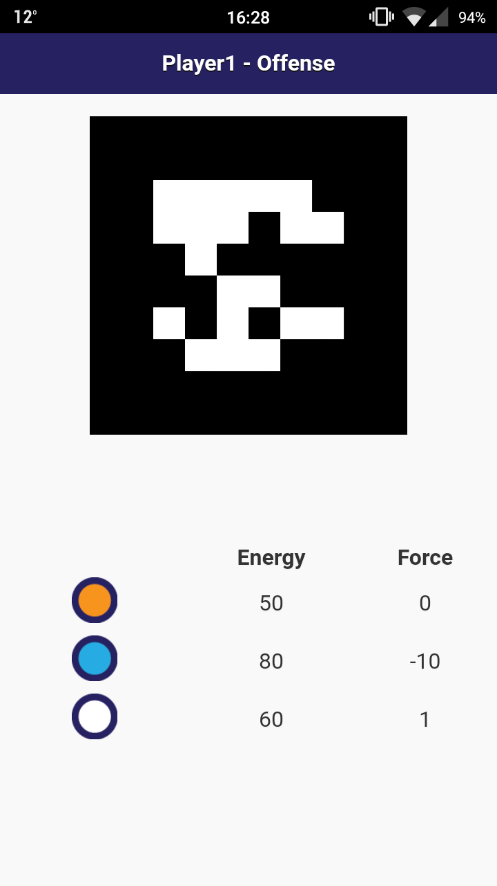
\includegraphics[width=0.60\linewidth]{images/c5/points.png} 
    \caption{The energy and force points of the swords.}\label{fig:5a}
  \end{subfigure}\hfill
  \begin{subfigure}[t]{0.48\linewidth}
    \centering
    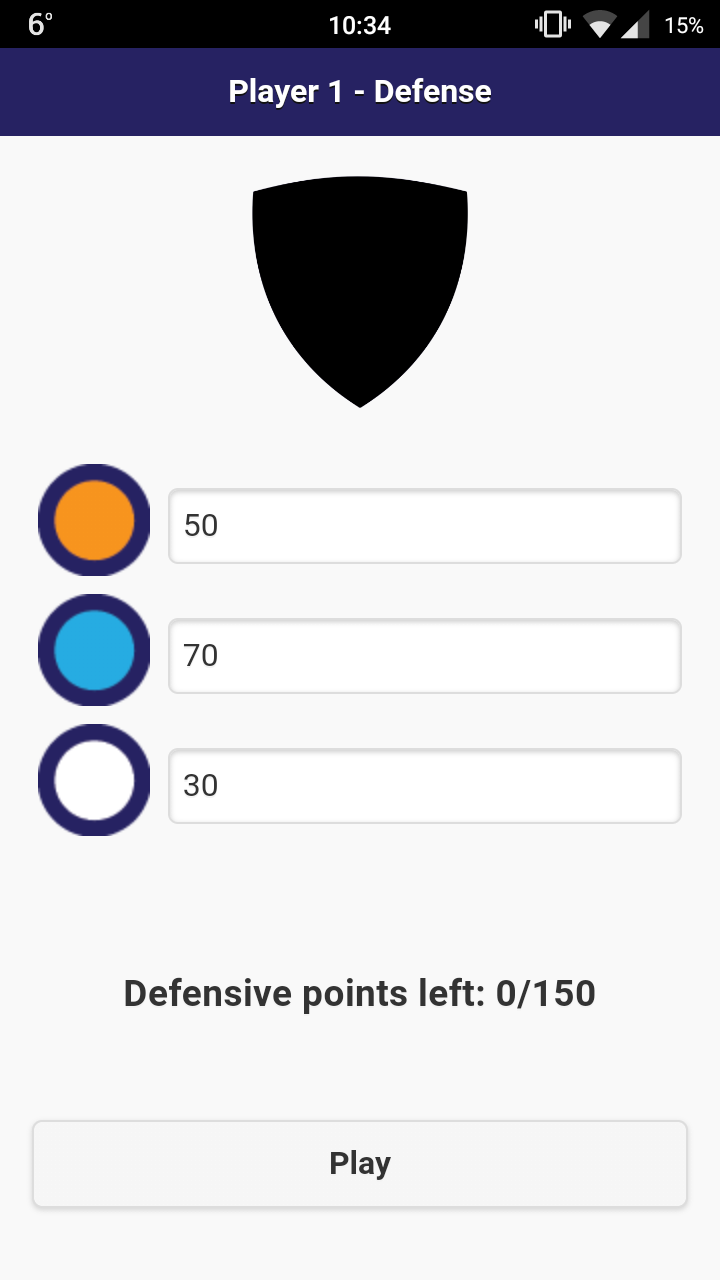
\includegraphics[width=0.60\linewidth]{images/c5/defense.png} 
    \caption{The defence points in the shields.}\label{fig:5b}
  \end{subfigure}
  \caption{The smartphone application}
\end{figure}

\subsection{Forging Shields}
The second phase is functional to the playability of the game and not strictly related to fostering \ac{CT} skills, even though it requires some analytical abilities. In this phase, the players must define their defensive strategies, which consist of allocating a number of defence points into three shields, each one corresponding to a different metal. The choice should be based on a couple of considerations: how the player guesses the opponent distributed force points on the different swords and which transformations have been chosen to build her own swords. For instance, if a player was not able to optimize the strategy for the steel sword, then she might consider allocating most defence points into the steel shield, in order to counterpoise her weak offensive strategy. To allocate defence points into the shields, each player interacts with a simple interface displayed on the smartphone (figure~\ref{fig:5b}).

\subsection{Enjoying the battle in VR}
The third phase of the game was designed to foster debugging capabilities, one of the main \ac{CT} skills highlighted in the literature. In the current version of TAPASPlay, however, this feature is limited to the visualization of the battle in \ac{VR}.

More precisely, when both the previous phases of the game are completed, a simple Android application showing a \ac{VR} video is made available from the server. Both players must wear VR goggles to enjoy the content of the video. The server provides each player with a different video on the basis of the scores it has received from the Web application. For instance, if player 1, who used the halo with blue hilts, reached the highest score, the video shows a knight wearing a blue armour defeating the opponent dressed in red; otherwise, a video with reversed roles is played. The \ac{VR} video shows two knights armed with sword and shield. In the beginning, a button with the ``Start'' label is visualized and a pointer placed at the centre of the user's sight suggests that gazing at it will allow playing the animation (figure~\ref{fig:6a}). After having pressed the button, the two knights approach the centre of the scene and, when they are close enough, they start duelling. They exchange a few hits for a little while, then the knight on the left takes a few steps back, runs toward the opponent and launches the decisive blow. The wounded knight falls on the ground and, while the winner cheers, a text appears on the background, confirming which player won (figure~\ref{fig:6b}).

Supporting this \ac{VR} visualization to inspect players' solutions provides an engaging way to visualise the outcome of the strategies and supports the learning of debugging capabilities within the gameplay\added[comment={D46}]{ by providing a way of tracking them}.

\begin{figure}[ht!] 
  \begin{subfigure}[b]{0.48\linewidth}
    \centering
    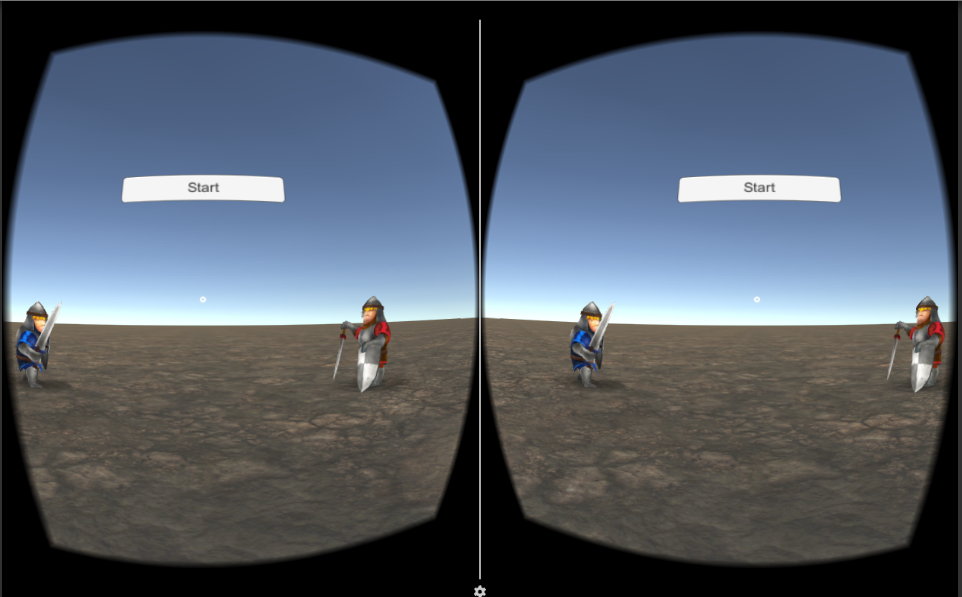
\includegraphics[width=1.02\linewidth]{images/c5/start-VR.png} 
    \caption{Beginning of a duel.}\label{fig:6a}
    %\vspace{4ex}
  \end{subfigure}\hfill
  \begin{subfigure}[b]{0.48\linewidth}
    \centering
    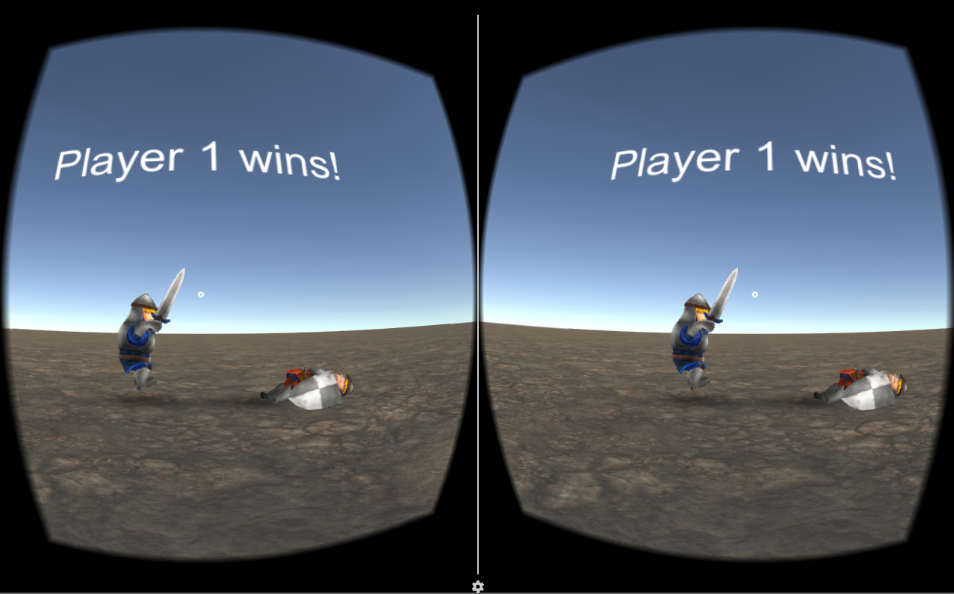
\includegraphics[width=1.02\linewidth]{images/c5/final-VR.png} 
    \caption{End of a duel: player 1 has won.}\label{fig:6b}
  \end{subfigure}
  \caption{Visualizing the battle in \ac{VR}.}
\end{figure}

\section{Evaluation}\label{sec:ev5}
This section presents the goals, hypotheses, and description of the experiment carried out to test TAPASPlay and address the Research Question stated in the introduction of this chapter, following the guidelines of the American Psychological Association~\cite{Wohlin:2000:ESE:330775}.

\subsection{Goals}
The goal of the experiment is to evaluate whether TAPASPlay \replaced[comment={D48}]{can be employed to develop \ac{CT} skills while providing a fun and enjoyable gameplay}{provides a fun and enjoyable experience to players while helping them develop \ac{CT} skills}. The purpose is to evaluate whether physical manipulation might foster \ac{CT} skills through gameplay in \ac{IL} domains.

\subsection{Research Questions}
User participation in system development can be effectively achieved by creating the conditions for their empowerment by supporting them in appropriating those \ac{CT} skills~\cite{Wing:2006iz} necessary for understanding and contributing to the system evolution.

Gameplay offers an opportunity to teach high-level \ac{CT} concepts indirectly in an engaging way to an ever wider audience, keeping them in a continuous Flow state.

In order to effectively teach \ac{CT} skills, gameplay should foster playful engagement and collaborative learning. \acp{TUI} exploit humans' innate dexterity for objects' manipulation to aid understanding of abstract concepts --- such as the ones involved by coding and \ac{CT}~\cite{turchi2017tapas}. Coupling them with gameplay also improves the playfulness~\cite{PRICE2003169}, relieving users from the mental burden carried by more artificial interaction paradigms.

One of the other benefits of \acp{TUI} is their natural predisposition towards collaboration, which is beneficial not only for learning in general but especially for fostering \ac{CT} skills~\cite{Wang:2014jy}. Moreover, it is also a distinctive trait of some of the most engaging games.

The Research Question derived from this context and addressed by this chapter is then: \textit{``Can physical objects manipulation provide a playful and engaging way of learning \ac{CT} skills through gameplay?''}.

\subsection{Experiment Design}
An exploratory research design was used, comprising oral feedback, observations, and a post-test survey.

\subsection{Participants}
The participants of the experiment were 18 UK secondary school female students of Key Stage 4 (15 years old) coming from different schools in the London area. None of them had a solid programming background, but a small subset (3 of them) had a little experience in block-based programming with Scratch. No prerequisite knowledge was required to perform the tasks, and none of the participants had prior knowledge of neither \ac{TAPAS} nor TAPASPlay. A brief introduction to the system and the game was provided to the experiment group.

\subsection{Settings and Experiment Tasks}
The study was conducted within the Brunel University London facilities, in a laboratory inside the Department of Computer Science, as depicted in figure~\ref{fig:studysetting}.

\begin{figure}
  \centering
  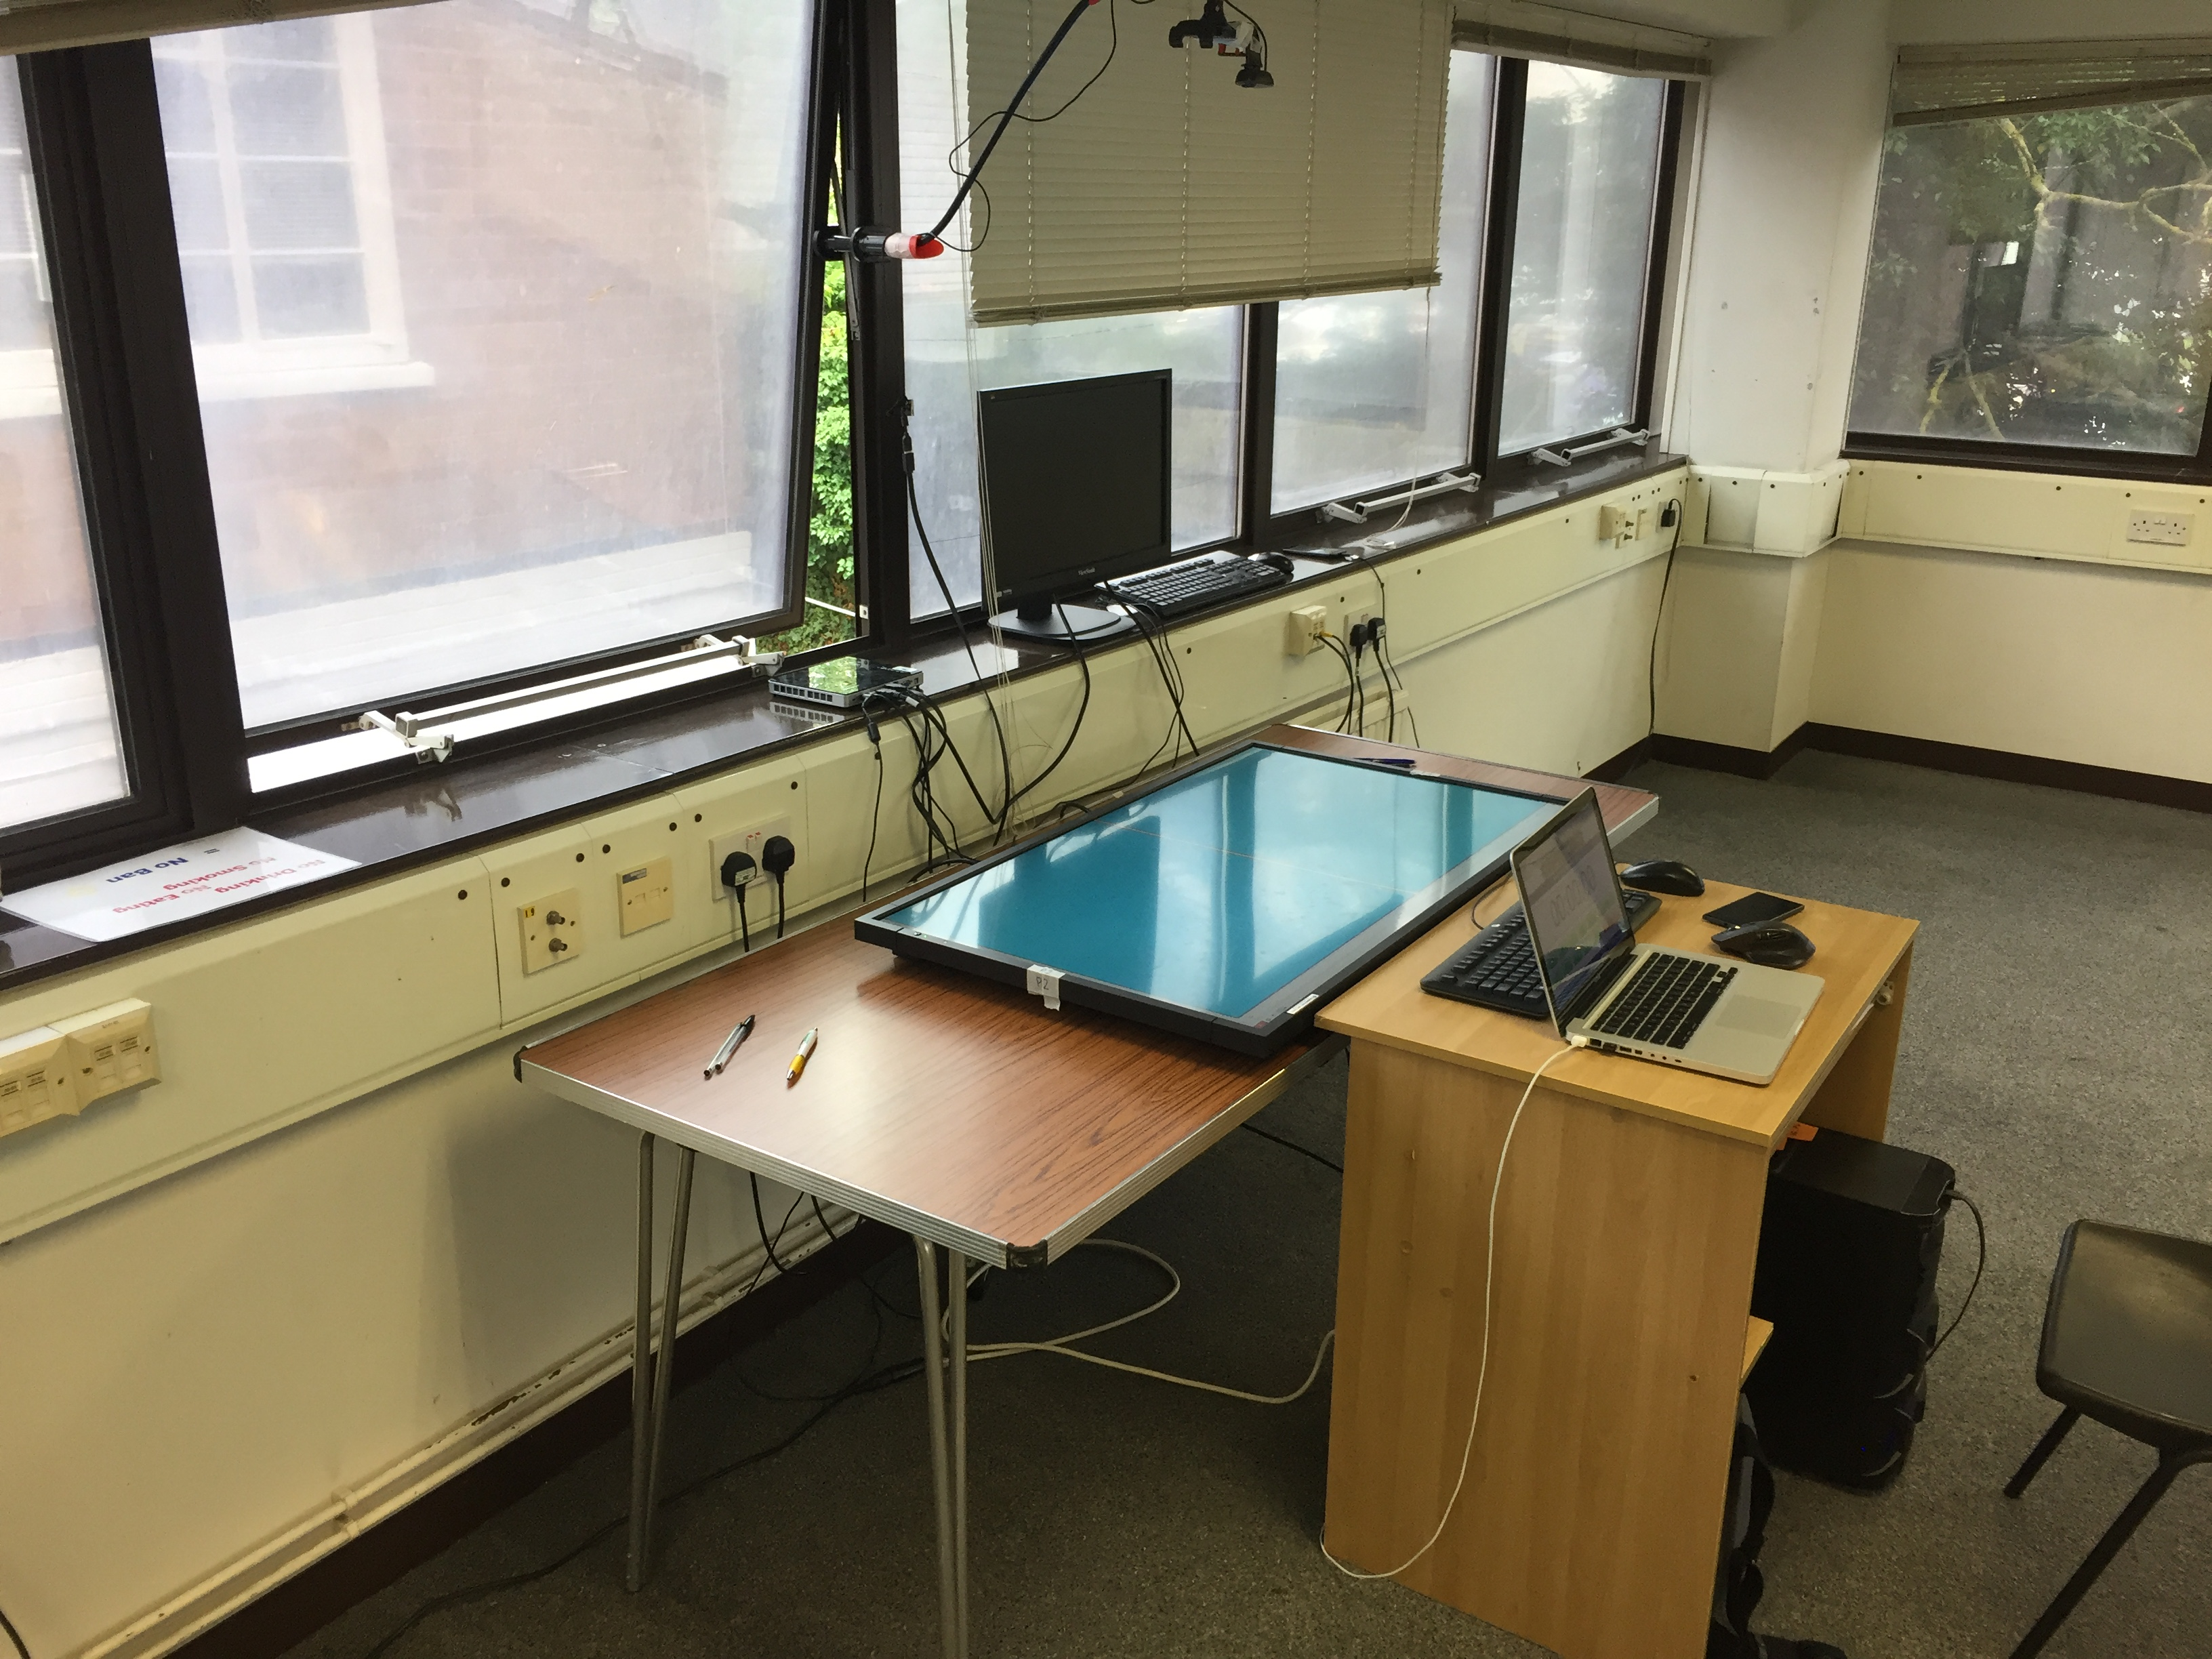
\includegraphics[width=.7\textwidth]{images/c5/study-setting.jpg}
  \caption{The study setting inside a university laboratory.}
  \label{fig:studysetting}
\end{figure}

Participants were presented with a prototype of TAPASPlay and tasked them with playing a single-turn game, i.e.~forging one sword each; the \ac{VR} visualisation and the defense strategy definition were purposively removed in order to focus the evaluation just on the proposed interaction and the effects of a \ac{TUI}-based gameplay on \ac{CT} skills in \ac{IL} domains.

The developed game scenario (i.e.~the available puzzle pieces at the beginning of a game, as depicted in table~\ref{tab:scenario}) was meant to provide players with many strategies and different difficulty levels. \replaced[comment={D49}]{This way participants could implement different strategies based on their skill level and progression throughout the game}{This allowed investigating over \ac{CT} level and progression throughout the game}.

Indeed, the puzzle shapes provide constraints and introduce conflict within the game: a player needs to maximise the force points of her sword while using the available puzzle pieces in an appropriate order. Moreover, each puzzle piece has a cost, and the sum of the puzzle pieces' cost that makes up a sword mustn't go over 100. The initial and final shapes were both triangular.

\begin{table}[ht!]
  \caption{The TAPASPlay scenario tested with participants.}
  \label{tab:scenario}
  \renewcommand{\arraystretch}{1.6}
  \newcounter{blocks}\newcommand\bnum{\stepcounter{blocks}\arabic{blocks}}
  \centering
  \begin{tabular}{lcccc}
    \cmidrule[\heavyrulewidth]{2-5}
    & Input Shape & Output Shape & Energy Cost & Force Points \\
    \cmidrule[\lightrulewidth]{2-5}
    \bnum: & $\bigcup$ & $\bigsqcap$ & 10 & $+8$ \\
    \bnum: & $\bigcup$ & $\bigwedge$ & 10 & $-9$ \\
    \bnum: & $\bigvee$ & $\bigcap$ & 5 & $\times (-1)$ \\
    \bnum: & $\bigvee$ & $\bigwedge$ & 20 & $\times 3$ \\
    \bnum: & $\bigvee$ & $\bigsqcap$ & 15 & $+13$ \\
    \bnum: & $\bigsqcup$ & $\bigsqcap$ & 5 & $+8$ \\
    \bnum: & $\bigsqcup$ & $\bigcap$ & 15 & $-12$ \\
    \bnum: & $\bigsqcup$ & $\bigwedge$ & 10 & $+10$ \\
    \bnum: & $\bigsqcup$ & $\bigsqcap$ & 10 & $+8$ \\
    \cmidrule[\heavyrulewidth]{2-5}
  \end{tabular}
\end{table}

\subsection{Procedure}\label{sec:procedure}
Participants were randomly clustered in 8 groups, 6 groups of 2 people each and 2 groups of 3, and the study was conducted in four different sessions, one for each individual game match played: one between the two teams of 3 people, and the rest between the other teams, paired in a randomised fashion.

All interactions with the tabletop surface and oral feedback provided during the game were recorded. At the end, a random participant from each group was asked to fill in a short questionnaire about her experience. Responses were given in terms of (Q1) enjoyment, (Q2) collaboration, and (Q3) interactivity, using a Likert scale from 1 (strongly disagree) to 5 (strongly agree) --- like well-known similar questionnaires (e.g., SUS~\cite{brooke1996sus}) --- with a neutral midpoint (neither agree nor disagree) in order to avoid directing the choices towards just negative or positive sentiments. The questionnaire presented the following statements:
\begin{enumerate}[label=Q\arabic*]
  \item I enjoyed playing TAPASPlay.
  \item I think TAPASPlay can be a fun game to play with friends.
  \item I enjoyed playing TAPASPlay on a tabletop by moving a smartphone.
\end{enumerate}

A 6 minutes average duration of each match was devised from an early internal playtesting phase of the game scenario. Each experimental session was then planned to last 15 minutes in total: 3 minutes for a brief explanation of how the game works and its rules, 2 minutes of practice, 8 minutes for the actual match, and 2 minutes to give feedback and fill in the questionnaire.

\subsection{Summary}
\added[comment={MP3, MP8, D43, D46}]{To recap, table \ref{tab:ch5summary} presents a summary of the specific \ac{CT} dimensions as defined in~\cite{Brennan:2012} examined in the evaluation, along with the related assessment approach, as reported in chapter \ref{chap:background}.}

\begin{table}[ht!]
  \caption{Summary of the specific \ac{CT} dimensions~\cite{Brennan:2012} considered by the evaluation with the related assessment approach.}\label{tab:ch5summary}
  \centering
  \begin{tabular}{M{0.2\linewidth}m{0.5\linewidth}M{0.2\linewidth}}
    \toprule
    \textit{\ac{CT} Dimension} & \textit{Description} & \textit{Assessment} \\
    \midrule
    Concept: sequences & Ex\-press\-ing a par\-tic\-u\-lar ac\-tiv\-i\-ty or task as a se\-ries of in\-di\-vid\-u\-al steps or in\-struc\-tions that can be ex\-e\-cut\-ed by the com\-put\-er. & Project Analysis \\
    Practice: being incremental and iterative & Changing the plan in response to approaching a solution in small steps. & Artefact-Based Interviews \\
    Practice: abstracting and modularizing & Building something large by putting together collections of smaller parts. & Design Scenarios \\
    \bottomrule
  \end{tabular}
\end{table}

\added{Moreover, this evaluation preliminarily investigated over the enjoyability (questionnaire's Q1), collaboration support (questionnaire's Q2), and interactivity (questionnaire's Q3) of the learning experience provided by TAPASPlay.}

\section{Results}
The collected data were analysed by
\begin{enumerate*}[label=(\arabic*)]
  \item performing a content analysis on the feedback,
  \item summarising the recorded game strategies employed by participants, and
  \item analysing the questionnaire results.
\end{enumerate*}
The findings are reported below.

\subsection{Feedback}
The overall response was positive, but participants needed some practice at first to get going assembling swords. Indeed, all the groups managed to play and successfully assembly a sword in the given time.

All groups were involved in playing the game, and all groups members were trying to work out the right sequence of pieces to assemble the strongest sword possible. All participants looked engaged in \replaced[comment={D51}]{the discussion with their peers, offering support and ideas to solve the problem}{in offering their support and ideas to solving the problem and actively discussing within their group}: none of the participants was left isolated from \replaced[comment={D52}]{their groups, regardless of size}{her group, even in largest ones (3 participants)}. \replaced[comment={D53}]{TAPASPlay fosters collaboration and stimulates discussion by having users around a table interacting with objects laying on it}{The collaboration aspect of TAPASPlay seemed to have properly worked to stimulate discussions and teamwork}.

A pointer received during the experiment was related to the proposed interaction modality. The \ac{TUI} seemed easily grasped and manoeuvred by participants, but the individual control point (i.e.\ the smartphone) and lack of support for mixed interaction (e.g., multi-touch) were pointed out by someone as the main hiccup to a better gameplay experience. Yet this promoted an off-the-screen collaboration where group members interact with each other to reach a decision, while in the end, one member took control of the smartphone on the tabletop surface. It fostered group discussion and kept all team members involved in the decision process, balancing the need of each member to experiment with her own ideas and contribute to the overall discussion.

Another point that was made from some participants during the study was related to the fall-back mechanism of TAPASPlay. A simple undo action, triggered with a button on the smartphone interface, detaches the latest piece that was attached to the current halo and puts it back to its original position on the board, redistributing the energy points consumed. Three groups used the undo action, while the others preferred discussing the strategies amongst themselves and act once they figured out the whole process, without experimenting it first. Designing an improved fall-back mechanism that properly represents the system status and capabilities across different heterogeneous devices with a \ac{TUI} is still an open question for Cross-Device interaction research~\cite{Houben:2017:OCC:3135412.3121348}. 

\subsection{Strategies}\label{sec:strategies}
A total of 10 complete strategies were produced by all the groups, as summarised in table~\ref{tab:strategies}: on the left the strategies are reported as ordered sequences of the puzzle pieces in table~\ref{tab:scenario} with their corresponding numbers, as they were assembled during the game; the number of groups that issued a strategy is reported on the right when greater than 1. Six groups completed a single strategy each and decided to end the game there, while the other two groups --- not playing in the same session --- kept experimenting further after completing one sword, and issued two complete strategies each: the first successfully completed strategies (b) and (d), while the second (e) and (f).

\begin{table}[ht!]
  \caption{The strategies completed by participating groups. On the left, numbers correspond to the puzzle pieces labelled in table~\ref{tab:scenario}, while on the right the number of times (when greater than 1) the corresponding strategy was issued during the study is reported.}\label{tab:strategies}
  \newcounter{strategies}\newcommand\snum{\stepcounter{strategies}\alph{strategies}}
  \centering
  \begin{tabular}{llc}
  \cmidrule[\heavyrulewidth]{2-3}
  (\snum) & $5 \to 8$ &  \\
  (\snum) & $5 \to 6 \to 8$ & $(\times 2)$ \\
  (\snum) & $5 \to 9 \to 8$ & $(\times 3)$ \\
  (\snum) & $5 \to 6 \to 9 \to 8$ & $(\times 2)$ \\
  (\snum) & $5 \to 9 \to 6 \to 8$ & \\
  (\snum) & $5 \to 9 \to 6 \to 8 \to 4$ & \\
  \cmidrule[\heavyrulewidth]{2-3}
  \end{tabular}
\end{table}

The average number of pieces used to complete a sword was 3.4, with a standard deviation of 0.8. The majority of the strategies issued were na\"{i}ve, in that they were built through a greedy algorithm using just a small number of pieces and without multiple trials (strategies (a), (b), and (c) in table~\ref{tab:strategies}), while the other strategies were a bit more complex and \added[comment={D54}]{sometimes }required more effort --- i.e.\ backtracking\added{, deferring completing a strategy directly and using more pieces to gain more points} --- to be discovered.

\subsection{Survey}
Lastly, the questionnaire was filled by a randomly chosen participant from each group, whose results are reported in table~\ref{tab:survey}.

\begin{table}[ht!]
  \caption{The survey results.}\label{tab:survey}
  \centering
  \fontsize{10}{11}\selectfont
  \begin{tabular}{cccccc}
    \toprule
    & Strongly Disagree & Disagree & Neither Agree nor Disagree & Agree & Strongly Agree \\
    \midrule
    Q1 & 0 & 0 & 3 & 3 & 2 \\
    Q2 & 0 & 1 & 2 & 4 & 1 \\
    Q3 & 1 & 0 & 0 & 4 & 3 \\
    \bottomrule
  \end{tabular}
\end{table}

All three statements proposed (section~\ref{sec:procedure}) were rated positively by the majority of respondents. The game interactivity (Q3) was the most positively perceived with an average score of 4, 5 out of 8 participants judged the enjoyment (Q1) more than neutral, with an average score of 3.875. The collaboration aspect of TAPASPlay (Q2) seemed to have been appreciated by most of the participants, with \replaced[comment={D55}]{three exceptions}{just one exception}, with an average score of 3.625.

\section{Discussion and Post-Hoc Analysis}
From the results of the study, the Research Question set out to be investigated in the introduction can be addressed.

First, the experience provided by TAPASPlay was received positively from participants: the feedback recorded during the game reports a positive reception from users, which is also confirmed by the survey results (Q1). Devising an engaging gameplay is fundamental in order to foster \ac{CT} skills, having to remove all the extra mental burden that comes from unnecessary game mechanics. \acp{TUI} provide a natural way of interacting with the game, without any artificial means of control, making the game easy to play and fun. TAPASPlay was also positively received in terms of interactivity, as evidenced by the survey results (Q3).

What is even more remarkable is that such results were achieved within a group of young girls, even though the game wasn't designed with this specific user group in mind: gender imbalance and under-representation have always been major issues affecting the Silicon Valley and the whole tech community in general, making it necessary to come up with new strategies to correct this phenomenon~\cite{tzafilkou2017gender,beckwith2006gender,Huff:2002:GSD:543812.543842,Cassell:1998:BMK:295056}. Engaging young girls in \ac{STEM} activities means empowering them with the right tools to actively participate and take control of the issues coming up in the future, allowing them to take on a more central role in the science and technology sector.

\replaced[comment={D56}]{The survey results report how TAPASPlay provides an engaging gameplay (Q1) using a \ac{TUI} that makes it a highly interactive experience (survey's Q3).}{The observed and reported participants engagement (survey's Q1) demonstrates how TAPASPlay provides a new way of fostering \ac{CT} skills through gameplay using a \ac{TUI} that allows a highly interactive experience (survey's Q3) and at the same time well-crafted game mechanics.}

Collaboration is yet another aspect worth discussing in more detail: TAPASPlay was designed from the ground up on top of \ac{TAPAS} to support collaboration in order to foster \ac{CT} skills. Indeed, Kazimoglu et al.~\cite{Kazimoglu:2012ft} report that socialization is another \ac{CT} skill fostered by learning through gameplay. The feedback obtained from participants and the results of the survey (Q2) confirm that TAPASPlay was well received as a collaborative game, stimulating discussions amongst teammates and fostering a stimulating learning environment. The gaming experience led users to socialize by continuously sharing thoughts about their approaches during the game, thus stimulating cooperative strategy development useful in co-design processes.

The lack of group members isolation is yet another benefit of the proposed gameplay observed during the study: softening the ``lone wolf'' effect --- described as the preference to work alone and dislike of group processes --- can positively affect team performance and improve learning~\cite{barr2005exploring}. Indeed, one can seldom observe an even participation in learning groups, especially big ones~\cite{Turchi:2015dr}, thus smoothing group participation level is a favourable consequence of balancing interaction style, groups activity and size.\added[comment={D57}]{ However, this effect will have to be validated further in future studies with larger groups size.}

Moreover, strategies issued by participating groups can be analysed to discuss how TAPASPlay fosters \ac{CT} skills: interestingly, the strategies adopted by the groups were quite different from each other, making use of a different amount of puzzle pieces \replaced[comment={D58}]{and of}{demonstrating support to} different algorithmic \replaced{strategies}{thinking} (improving from a greedy strategy to backtracking). This, depending on the developed scenario, can provide the right conditions for supporting \ac{CT} skills at different levels, allowing players to assembly different strategies and reach for the hardest ones to build as their skills progress (i.e.\ low floor, high ceiling~\cite{Repenning:fy}).

Another result worth pointing out is what happened to the two groups that issued more than one strategy (section~\ref{sec:strategies}). The first one assembled strategy (e) in table~\ref{tab:strategies}, then (f); this progression is evidence of a divide-et-impera approach, i.e.\ the result of decomposing a strategy into subproblems and recursively solve them: once the problem has been solved with the first strategy, the group recognised that the solution could be extended by adding an extra piece, gaining more points.

Next, the second one assembled strategy (b) in table~\ref{tab:strategies}, then (d); perhaps even more deeply than before, this progression is evidence of abstracting the building of a sword and recognising that another piece can be added without changing the input and output of the whole strategy, thus completing it and gaining more points.

The rationale behind the design of TAPASPlay also provides \deleted[comment={D59}]{with }other pointers towards fostering \ac{CT} skills, stemming from its design. TAPASPlay detaches composition from execution~\cite{turchi2017tapas} by offering two different interaction styles and tools: puzzle-based interaction on a tabletop display and a smartphone are used for composing the strategy (problem-solving); whilst\replaced[comment={D60}]{ \ac{VR} to support and make more exciting checking solution execution}{, \ac{VR} is adopted for checking solution execution}. This mechanism fosters the design-debug-run stages, three key aspects of \ac{CT}~\cite{Kazimoglu:2012ft}, or in other terms, the process of problem formulation-solution expression-execution and evaluation~\cite{Repenning:fy}.

Moreover, while automation is supported by \ac{VR}, analysis, abstraction and problem decomposition are types of reasoning that players are supposed to apply when trying to maximize the force points, under the constraints represented by shapes and limited energy points. As a matter of fact, the choice of displaying all transformations together at the beginning of a game makes \added[comment={D61}]{it }deliberately complex for the player to formulate a straightforward solution. On the other hand, if the player is ``lazy'' and does not want to apply a methodic decomposition process, but merely tries to satisfy the constraints (i.e.\ greedy strategy), a solution would be reached, but chances are that it won't be a good one in terms of force points. Therefore, the player will try to ``fix it'' by analyzing it and identifying the weakest subsequence of transformations. Hence, the solution would be reformulated by replacing the poor part with a different sequence of pieces (i.e.\ backtracking). This process might be repeated several times, inducing the player to iteratively apply the model of \ac{CT} process proposed in~\cite{Repenning:fy}.

All these skills are indeed crucial for the end-users to play an active role in the algorithmic solution proposed and discussed with technologists, therefore enhancing the formers' active participation to system development and evolution, aiding them in understanding and selecting the right solution while helping them modelling the problem.

\section{Threats to Validity}
There are several validity threats to the design of this study.

\paragraph{Internal Validity} The limited number of participants allowed to properly reason about different effects found during the study, but a more extended experiment testing all the game phases with more users needs to be designed in order to properly validate \deleted[comment={D62}]{the survey results and }the effects over isolation of team members, which cannot be definitive yet. The experimenter effect is concerned with any biasing effects in a study that is due to the actions of the researcher. The researcher attempted to carry out the study as objectively and as accurately as possible, acting as an observer limited to recording feedback\added[comment={D50}]{, but the survery responses might be affected}. The subject effect could have determined changes in the participants' behaviour due to being in the study and under observation; in this case, the study was carried out within a traditional learning environment during a series of workshops with similar game activities.

\paragraph{External Validity} The sample was a group of only female students coming from different schools of the London area, which was a proper starting point to validate engagement in an under-represented group within the tech industry, but in extending this work TAPASPlay should be tested with a more diverse and international user group to investigate different effects. The lack of a mixed modality which fosters on-screen collaboration and support for an advanced fall-back mechanism limited in-game experimentation and prevented certain uses which might have affected the observed results.

\paragraph{Construct Validity} Due to experiment time lim\-i\-ta\-tions, the post-test ques\-tion\-naire was filled by a ran\-dom member of each group and was limited to three questions designed to measure different aspects of the experience. This, together with the limited number of respondents, might have affected the results, even though the survey results weren't used alone, but rather cross-referenced them with the in-game oral feedback from participants.

\section{Contributions}
Parts of the work and results described in this chapter have been previously published in\added[comment={MP6}]{ the following}:
\begin{itemize}
  \item \added{The Design of TAPASPlay described in section \ref{sec:tapasplay} has been published in}~\cite{malizia2017eudtapasplay,malizia2017vltapasplay,fogli2017sustaining}.
  \item \added[comment={MP6}]{The Evaluation of TAPASPlay reported in section \ref{sec:ev5} and its Design in section \ref{sec:tapasplay} have been published in~\cite{turchi2019collaborative}}.
\end{itemize}

\section{Conclusion}
The growing interest in \ac{CT} is witnessed by very recent literature~\cite{Yadav:2017ir}, which describes how \ac{CT} is becoming more and more important in student and teacher education. In this chapter, \ac{CT} skills are shown to be fundamental to allow end-users to collaborate to system design and evolution at use time. For this reason, contrarily to other block-based approaches, in TAPASPlay blocks do not represent programming statements (like for example, the ``if-then'' block in Scratch) but remain at a higher level of abstraction, to promote problem decomposition abilities rather than programming ones.

Like \ac{TAPAS}, TAPASPlay considers \acp{TUI} and physical object manipulation fundamental tools to make user activities more engaging. Indeed, it has been demonstrated that tangible programming has the potential to help children cultivate skills such as abstraction and problem decomposition~\cite{Wang:2014jy}.

In this chapter the design rationale behind TAPASPlay was presented, a turn-taking serious game using gameplay to foster \ac{CT} skills by making learners experience engaging and social. In particular, it contributes to the research trend that explores learning through gameplay~\cite{Kazimoglu:2012ft} --- instead of learning through designing systems --- in fostering \ac{CT} skills. The prototype was employed in a study with a group of secondary school girls that investigated the effects of physical objects manipulation on learning \ac{CT} skills through gameplay. The results showed some evidence that TAPASPlay offers an engaging and playful environment to develop \ac{CT} skills.

TAPASPlay is, however, a first \replaced[comment={D63}]{attempt at fostering \ac{CT} skills of end-users through gameplay}{proposal to fostering \ac{CT} skills of end-users}. Further experiments testing all three game phases with different user groups and game scenarios will be carried out \deleted{in the next future }to demonstrate the validity and robustness of the idea. Furthermore, several extensions of TAPASPlay have been already planned, in order to tailor the system to end-users' characteristics and introduce different levels of complexity in the game. At the moment, only a \ac{VR} simulation of the battle is available as an outcome of the game; however, the system could be extended adding a more interactive functionality that better resembles the debugging activity, in which players can compare step-by-step how they built their swords and eventually see what was the optimal solution.

The next chapter concludes the thesis by summarising the results in light of the original Research Question to be addressed, recaps the contributions and implications, and discusses possible future research directions.